%Wir verwenden eine DIN-A4-Seite und die Schriftgröße 12.
\documentclass[a4paper,12pt]{scrartcl} 


%Diese drei Pakete benötigen wir für die Umlaute, Deutsche Silbentrennung etc.
%Apple-Nutzer sollten anstelle von \usepackage[latin1]{inputenc} das Paket \usepackage[applemac]{inputenc} verwenden
%% \usepackage[latin1]{inputenc}
%%apt-get install texlive-lang-german damit ngerman keine Probleme mehr macht !!
%\usepackage[utf8]{inputenc} 
%\usepackage[T1]{fontenc}
%\usepackage[ngerman]{babel}

%Das Paket erzeugt ein anklickbares Verzeichnis in der PDF-Datei.
%\usepackage{hyperref}

%Das Paket wird für die anderthalb-zeiligen Zeilenabstand benötigt
\usepackage{setspace}

%%HTWM-Vorlage - benoetigt apt-get install texlive-fonts-extra
\setcounter{tocdepth}{3}				%Schatelungstiefe Inhaltsverz.
\usepackage[utf8]{inputenc}			%deutsche Umlaute
\usepackage{german, ngerman}
\usepackage[ngerman]{babel}			%Rechtschreibprüfung
\usepackage{color,listings} 			%Quellcode Highlighting, bindet das
%Paket Listings ein
\usepackage{listings}
\usepackage{color}
\usepackage{textcomp}
\usepackage[T1]{fontenc}				%srccode
\usepackage[scaled]{beramono}		%srccode
\usepackage{longtable}				%mehrseitige tabellen
\usepackage[tableposition=b]{caption}
\usepackage[pdftex, pdftoolbar=false, hyperfootnotes=false, bookmarks,
bookmarksopen, bookmarksnumbered, bookmarksopenlevel=2, pdfpagelabels=true,
pdfstartpage=3, pdfstartview=FitH,]{hyperref} %Verlinkungen
\usepackage{array}					%farbige Tabellen
\usepackage[table]{xcolor} 			%farbige Tabellen
\usepackage{graphicx}				% \includegraphics bnoetigt dies
\usepackage{subfigure} 				%% Bilder nebeneinander einfuegen

\usepackage{fancyhdr, graphicx}		%% Logo auf Titelseite
\renewcommand{\headrulewidth}{0pt}
\fancyhead[L]{}
\fancyhead[R]{
  
\includegraphics[width=52mm]{./images/htwk.png}
}

\usepackage{draftwatermark}			% wasserzeichen
	%Quelle: http://choorucode.com/2010/05/05/latex-adding-draft-watermark/?like=1&source=post_flair&_wpnonce=1c9f85538d
\SetWatermarkText{VORABVERSION}		% wasserzeichen-text
\SetWatermarkLightness{0.9}			% wasserzeichen-kontrast
\SetWatermarkScale{2.5}				% wasserzeichen-zeichengroe\ss{}e

\usepackage{float}					% Bilder mittels H-Paramter genau positionieren
\restylefloat{figure}				% Bilder mittels H-Paramter genau positionieren


\definecolor{Navy}{rgb}{0,0,0.5}
\definecolor{Gray}{gray}{0.5}
\definecolor{dunkelgrau}{rgb}{0.8,0.8,0.8}
\definecolor{hellgrau}{rgb}{0.95,0.95,0.95}
\definecolor{hellgrau2}{rgb}{0.93,0.93,0.93}

\hypersetup{
	colorlinks=true, 			% false: boxed links; true: colored links
	linkcolor=Navy,          		% color of internal links
	citecolor=Gray,        			% color of links to bibliography
	filecolor=magenta,      		% color of file links
	urlcolor=blue,           		% color of external links
	linkbordercolor={1 1 1}, 		% set to white
	citebordercolor={1 1 1} 		% set to white
}


%Einrückung eines neuen Absatzes
\setlength{\parindent}{0em}

%Definition der Ränder
\usepackage[paper=a4paper,left=30mm,right=30mm,top=30mm,bottom=30mm]{geometry}

%Abstand der Fussnoten
\deffootnote{1em}{1em}{\textsuperscript{\thefootnotemark\ }}

%Regeln, bis zu welcher Tiefe (section,subsection,subsubsection) Überschriften angezeigt werden sollen (Anzeige der Überschriften im Verzeichnis / Anzeige der Nummerierung)
%\setcounter{tocdepth}{3}
%\setcounter{secnumdepth}{3}

\fancypagestyle{htwkheader}
{
  \fancyhf{}	% clear all header and footer fields
    \fancyhead[RO]{
	\makebox[\textwidth]{	%% schiebe Logo nach aussen auf den Rand
		\rule{0.9				%% nach aussen schieben hoeherer Wert -> Logo weiter nach aussen
		  \textwidth}{0cm} %% nicht nach unten schieben = 0cm
			\includegraphics*[width=52mm]{./images/htwk.png}	%%Logo HTWK
	  }
  }
}


\begin{document}
%Beginn der Titelseite

\begin{titlepage}
%%\thispagestyle{htwkheader}		
%\addtolength{\voffset}{-2cm}		
%\addtolength{\topmargin}{-2cm}
%\addtolength{\bottommargin}{2cm}
%%%%%%%%%%%%%%%%%%%%%%%%%%%%%%%%%%%%%%%%%%%%%%%%%%%%%%%%%%
%%  Oberer Teil: Links Textblock HTWK, Rechts Logo HTWK %%
%%\begin{figure}[htbp]
%%\begin{minipage}[t]{6cm}	%% linker Teil
%%\vspace{0cm}
HTWK Leipzig\\
Fachbereich IMN \\
Wintersemester 2012/2013
%%\end{minipage}
%%\hfill						%% Zwischenraum auffuellen
%%\begin{minipage}[t]{6cm}	%% rechter Teil
%%\vspace{0pt}
%%\makebox[\textwidth]{	%% schiebe Logo nach aussen auf den Rand
%%  \rule{1				%% nach aussen schieben hoeherer Wert -> Logo weiter nach aussen
%%    \textwidth}{0cm} %% nicht nach unten schieben = 0cm
%%      \includegraphics*[width=52mm]{./images/htwk.png}	%%Logo HTWK
%%}

%%  \end{flushright}
%%\caption{Bild1}			%% keine Bildbeschriftung fuer Logo
%%\label{fig:Bild1}			%% nicht ins Abbildungsverzeichnis aufnehmen
%%\end{minipage}
%%\end{figure}

%\vspace{6cm}

%\addtolength{\voffset}{0cm}

\begin{center}
\begin{Large}
\vfill {\textsf{\textbf{
Beleuchtungssteuerung mit dem Mikrocontroller LPC1768
\\--VORABVERSION--\\
}}}
\end{Large}
Beleg im Fach Mikrocontrolleranwendungen
\end{center}

\begin{small}
\vfill
Marcel Kirbst, B.Sc.\\
Sieglitz 39 \\
06618 Molau \\
marcel.kirbst@stud.htwk-leipzig.de\\
\\
Sebastian Krause, B.Sc.\\
Dante-Stra\ss{}e 16 \\
04159 Leipzig \\
sebastian.krause@stud.htwk-leipzig.de\\
\\
\today
\end{small}

\end{titlepage}
\addtolength{\voffset}{0cm}

%%%%%%%%%%%%%%%%%%%%%%%%%
%%%Ende der Titelseite%%%
%%%%%%%%%%%%%%%%%%%%%%%%%

%Inhaltsverzeichnis (aktualisiert sich erst nach dem zweiten Setzen)
\tableofcontents

%Beginn einer neuen Seite
\clearpage

%Anderthalbzeiliger Zeilenabstand ab hier
\onehalfspacing

%%\pagestyle{plain}
%\pagestyle{headings}	%% lebende Kopfzeile

%%Abbildungsverzeichnis hier erstellen
\clearpage
\listoffigures

\clearpage
\section{Einleitung}
%%\pagestyle{empty}
Dieser Beleg befasst sich mit der Helligkeitssteuerung von Leuchtmodulen durch den Mikrocontroller LPC1768 in Verbindung mit dem PWM-Treiber PCA9685. Bei den
Leuchtmodulen handelt es sich um Baugruppen die mit jeweils sechs 1-Watt LEDs best\"uckt sind und \"uber eine integrierte Transistor-Endstufe versorgt
werden. Weiterhin soll ermittelt werden wie die Aussteuerung der einzelnen PWM-Stufen mit der real messbaren Beleuchtungsst\"arke korreliert. 
%% BILD:
\begin{figure}[htb]
  \begin{center}
%%    \includegraphics[width=1\hsize]{./images/foto_hardware_komplett.png}
    \includegraphics[width=1\hsize]{./images/foto_hardware_komplett_dunkel.png}
  \end{center}
\caption[\"Ubersicht der eingesetzten Hardware, Quelle: Autoren]{\label{fotohwuebersicht}\"Ubersicht der eingesetzten Hardware.}
\end{figure}

\clearpage
\section{Grundlagen}

Dieser Abschnitt führt einen kurzen \"Uberblick \"uber die für das Projekt nötigen theoretischen Grundlagen aus. Dabei wird auf Charakteristika der
Beleuchtungsmessung sowie verwendete Protokolle eingegangen.

\subsection{I2C Protokoll}

Der I2C-Bus ist ein von der Firma Philips entwickeltes Protokoll, welches zur Kommunikation zwischen Bausteinen und Baugruppen innerhalb von Ger\"aten
entwickelt wurde und auch unter dem Namen TWI firmiert. Wie der Name bereits andeutet handelt es sich um ein Bussystem, bei welchem die Daten seriell und
synchron \"ubertragen werden. Im Standard-Mode wird eine \"Ubertragungsrate von 100 KBit/S erreicht, es sind bei Vetrwendung anderer \"Ubertragungsmodi jedoch
auch \"Ubertragungsraten von bis zu 3,4 MBit/S m\"oglich. An einem I2C-Bus finden sich immer mindestens ein Master und bis zu 127 Slaves.

F\"ur weiterf\"uhrende Informationen sei an dieser Stelle auf die Spezifikationen des I2C-Busses verwiesen, welche unter \cite{speci2c} abrufbar
sind.

\subsection{OneWire Protokoll}
Als OneWire wird ein Bus-Protokoll bezeichnet welches nur eine Verbindungsleitung zwischen den Kommunikationspartnern erfordert, wenn diese ein gemeinsames
Masse-Potential haben. \"Uber diese Verbindungsleitung erfolgt sowohl die Spannungsversorgung als auch der Datenaustausch. OneWire arbeitet dabei asynchron,
dass hei\ss{}t es wird kein Taktsignal f\"ur die Kommunikation ben\"otigt. Die Daten\"ubertragung erfolgt bei einem OneWire-Bus im bidirektionalem
Halbduplexverfahren, dass hei\ss{}t es wird f\"ur das Senden und das Empfangen der gleiche Datenkanal benutzt, wobei aber immer nur gesendet oder empfangen
werden kann. Weiterf\"uhrende Informationen zum OneWire-Busprotokoll k\"onnen unter \cite{spec1wire} abgerufen werden.

\subsection{Beleuchtungsmessung}
Sebastian

\section{Eingesetzte Hardware}
In diesem Abschnitt soll kurz auf die einzelnen Komponenten des Messaufbaus eingegangen werden um dem Leser einen Überblick zu verschaffen und gegebenenfalls auf weiterführende Quellen zu den einzelnen Komponenten zu verweisen.

\subsection{CARALUX LED Control Board v1.1}
%Sebastian
%- grundlegende Plattform
%- von elmicro designed
%- Zweck: ansteuerung eines LED-Straßenlampenmoduls mit 16 LED-Modulen
%- Enthält Sockel für Mikrocontroller, pinkompatibel mit LPC1768
%- 16 Kanal PWM-Controller
%- Temperatursensor
%- betrieben mit 24 volt
%- Kommunikationsschnittstellen: USB, Ethernet

Das LED-Board als zentrale Komponente des Messaufbaus sowie auch der Lampe ist eine Entwicklung der Firma Elmicro für die Firma Caralux. Dieses LED-Board, das
für den Messaufbau in der Version 1.1 zur Verfügung stand, besitzt Schnittstellen für USB und Netzwerk, sowie über Schraubklemmen Anschlüsse für die
Energieversorgung mit 24 Volt, RS485 sowie für den Anschluss von 16 LED-Modulen. Die LED-Module werden jeweils über drei Leitungen vom LED-Board mit Masse, 24
Volt Versorgungsspannung sowie dem PWM-Signal, welches die Werte 0 Volt oder 5 Volt annehmen kann, versorgt.

Das LED-Board ist weiterhin mit einem PWM-Controller PCA9685 sowie einem Temperatursensor DS1820 bestückt und besitzt einen Sockel für den Mikrocontroller LPC1768.

\subsection{LED-Module und Optiken}
Die eingesetzten LED-Module wurden von der Firma Caralux gefertigt und tragen die Bezeichnung LED-LL-1,0/6L-DIM. Die Versorgungsspannung der LED-Module
betr\"agt 24 Volt bei einer maximalen Stromaufnahme von 0,35 Ampere. Weiterhin besitzen die LED-Module einen invertierten Signaleingang um die Helligkeit per
PWM-Signal zu dimmen, wobei die Signaleingangsspannung zwischen 0 und 5 Volt variieren darf und 0 Volt am Signaleingang zur maximalen Helligkeit des Moduls
f\"uhren. 

\begin{figure}[htb]
\begin{center}
  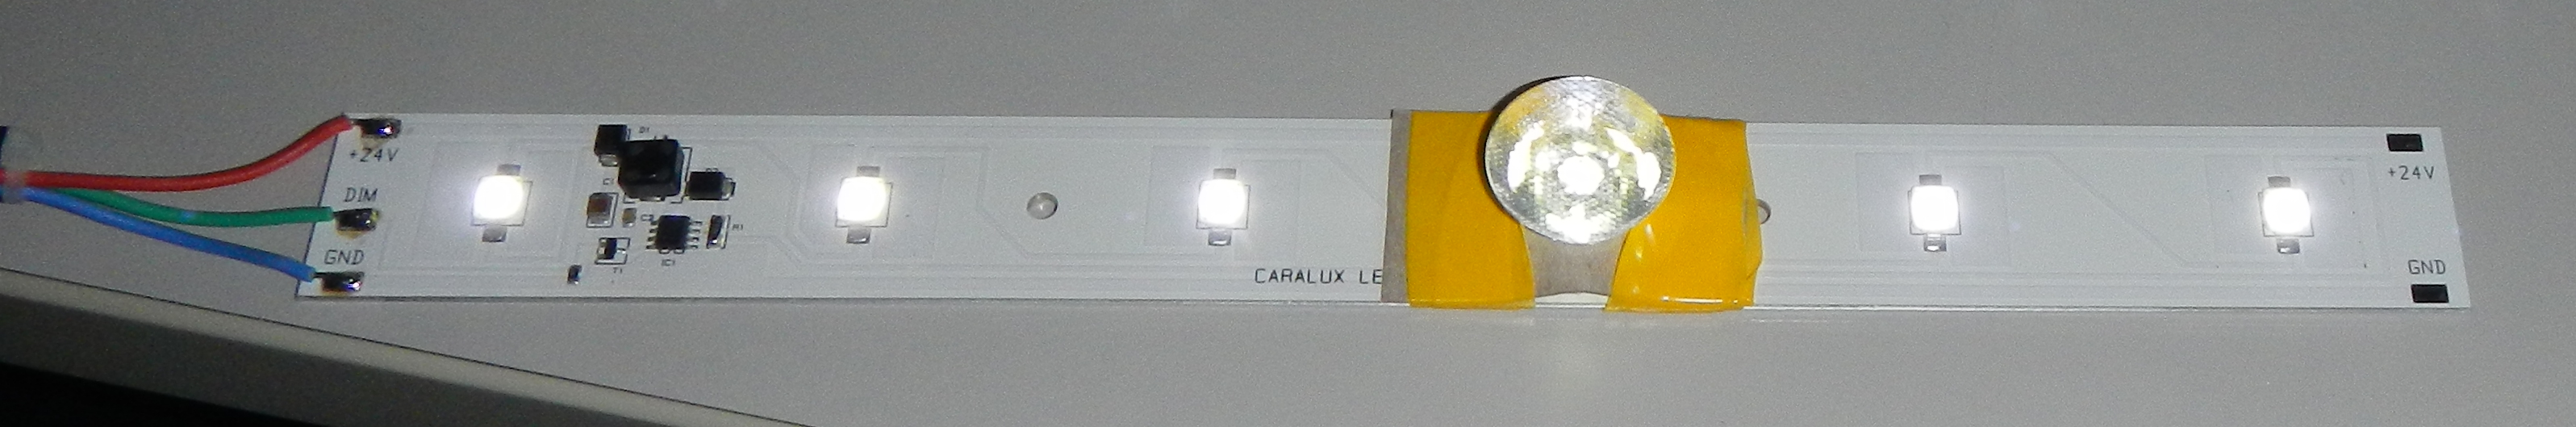
\includegraphics[width=1\hsize]{./images/foto_hardware_ledmodul.png}
\end{center}
\caption[LED-Modul der Firma Caralux mit provisorisch fixierter Optik im Messaufbau, Quelle: Autoren]{\label{fotohwledmodul}LED-Modul mit provisorisch fixierter
Optik f\"ur Einsatz im Messaufbau.}
\end{figure}
Die LED-Module sind jeweils mit sechs wei\ss{}en LEDs LUW W5AM-LX-6Q der Firma Osram best\"uck, die eine Farbtemperatur von 6500K aufweisen. Weitere Informationen zu diesem LED-Typ k\"onnen aus dem zugeh\"origen Datenblatt entnommen werden, welches unter \cite{specled} abgerufen werden kann. Durch die hohe
Leistungsaufnahme der LED-Module sollten diese ohne zus\"atzliche K\"uhlelemente nur f\"ur sehr kurze Zeitr\"aume in Betrieb genommen werden.

Die LED-Module sind so konstruiert das diese mit verschiedenen Optiken versehen werden k\"onnen um die Abstrahlcharakteristik jeder einzelnen LED variieren zu
k\"onnen. Im Messaufbau wurden Messreihen f\"ur die Optiken Titanium-O-M und Titanium-O-SS aufgenommen.
\begin{figure}[htb]
\begin{center}
  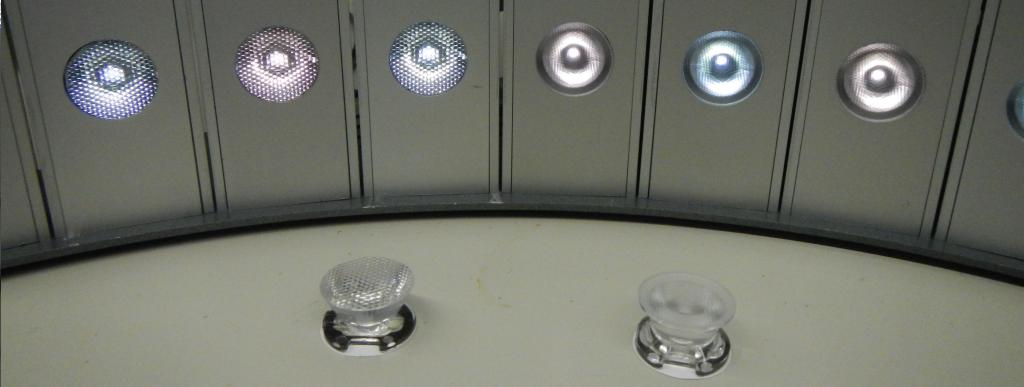
\includegraphics[width=1\hsize]{./images/foto_hardware_optiken.png}
\end{center}
\caption[LED-Optiken, links: Titanium-O-M, rechts Titanium-O-SS, Quelle:
Autoren]{\label{fotohwoptiken}LED-Optiken, links: Titanium-O-M, rechts Titanium-O-SS, Quelle:
Autoren}
\end{figure}
Die LED-Optiken besitzen einen Fuss, der an das LED-Modul angepasst ist. Weiterhin sind die LED-Optiken an der Unterseite mit doppelseitigem Kelebematerial
versehen, was eine leichte Fixierung auf dem LED-Modul erm\"oglicht.

\subsection{Mikrocontroller LPC1768}
Den Kern des Projekts bildet die Mikrocontrollerbaugruppe "`mbed LPC1768"' der
Firma NXP. Diese Baugruppe basiert auf einem ARM Cortex-M3, welcher umfangreiche
Austattungsmerkmale bietet und auf geringen Energieverbrauch hin optimiert ist.
Der LPC1768 kann mit einer Taktrate von bis zu 100 MHz betrieben werden und
bietet je nach Konfiguration bis zu 512 KByte Flash und bis zu 64 KByte
Datenspeicher. Weiterhin stehen umfangreiche Schnittstellen zur Verfügung um
Peripherie anbinden zu können, beispielsweise eine Ethernet-Schnittstelle, ein
USB-Anschluss, zwei CAN-Kanäle, drei I2C-Kanäle und weitere. Detailierte
Spezifikationen können dem Datenblatt entnommen werden, welches unter
\cite{speclpc1768} abgerufen werden kann.

\subsection{PWM-Controller PCA9685}
%%Anm.: Werte im Text in \texttt{WERT} schreiben, damit diese im Text als "Schreibmaschinenschrift" hervorgehoben sind, liesst sich besser ;)
Der verwendete PCA9685 ist ein programmierbar PWM-Controller mit 16 Kanälen und einer Auflösung von 12 Bit. Angesteuert wird dieser Controller über das 
Bus-Protokoll I2C. Durch sechs vorhandene Adresspins können bis zu 62 PCA9685 an einem Bus betrieben werden. Des Weiteren ist es möglich alle am Bus
befindlichen Controller gleichzeitig über eine All-Call-Adresse anzusprechen sowie zu konfigurieren. Zusätzlich können mittels 3 verschiedener Sub-Call-Adressen
auch verschiedene Gruppen von PWM-Controllern definiert werden. Über einen separaten OE-Eingang ist es möglich die Ausgabe der PWM-Kanäle komplett an- und
abzuschalten.

Die Konfiguration des PCA9685 erfolgt über acht Bit große Register. Tabelle \ref{tab:registers} listet diese in den entsprechenden Gruppen auf. 

\begin{longtable}{p{45mm}>{\columncolor[gray]{0.97}}p{25mm}p{65mm}}
\rowcolor[gray]{.9}
\textbf{Register} & \textbf{Adresse} & \textbf{Verwendung} \\ 
MODE1, MODE2 & 00h, 01h & Enhält allgemeine Parameter für den Betriebsmodus \\ 
\rowcolor[gray]{.95}
SUBADR1 - SUBADR3 & 02h - 04h & Definition der Sub-Call-Adressen \\ 
ALLCALLADR & 05h & Definition der All-Call-Adresse \\ 
\rowcolor[gray]{.95}
LED-Register & 06h - 45h & Separate Konfiguration der PWM-Kanäle \\ 
ALLLED-Register & FAh - FDh & Gemeinsame Konfiguration der PWM-Kanäle \\ 
\rowcolor[gray]{.95}
PRESCALE & FEh & Konfiguration der PWM-Frequenz mittels Prescaler \\ 
\caption{Konfigurationsregister des PCA9685}
\label{tab:registers}
\end{longtable}

Hierbei ist zu beachten, dass jeder PWM-Kanal mit vier Registern konfiguriert wird. Je zwei Register beinhalten einen zwölf Bit großen Wert für An- und 
Abschaltzeitpunkt innerhalb eines 4096 Schritte großen Zyklus. Soll also die erste Hälfte der PWM-Periode einen High-Pegel liefern, so beträgt der Einschaltwert
\texttt{0} und der Ausschaltwert \texttt{2047}. Analog dazu verhält sich das ALLLED-Register mit dem Unterschied, dass dieses Schaltverhalten auf alle Kanäle
abgebildet wird.

\subsection{Lichtsensor GeoSys GSLx}
Der zunächst verwendete Lichtsensor ist der GSLx der Firma GeoSys. Dieser besteht aus zwei Hauptkomponenten. Zum einen der eigentliche Sensor, welcher die Photodiode TSL250R des Herstellers Taos ist, sowie einen IC zur Verstärkung des Ausgangsstroms. Abhängig vom gemessenen Ausgangsstrom, welcher im Bereich von 5 - 20 mA liegt, kann somit die Beleuchtungsstärke ermittelt werden. Die laut Hersteller angegebene maximal messbare Beleuchtungsstärke liegt bei 50 Lux. Im Versuch stellte sich jedoch eine Beleuchtungsstärke von ca. 200 Lux als maximal erfassbar heraus.

TODO: Schaltung einfügen.

\begin{figure}[htb]
\begin{center}
%  
\includegraphics[width=0.5\hsize]{./images/htwk.png}
\end{center}
\caption[Teilschaltung zur Ansteuerung des GSLx, Quelle: Autoren]{\label{fig:schaltungGSLx}Teilschaltung zur Ansteuerung des GSLx}
\end{figure}

Die eingesetzte Konfiguration aus Mikrocontroller und Control Board bieten weder eine geeignete Spannungsquelle im zugelassen Bereich von 12 - 15 V noch eine Schnittstelle zur Erfassung des Ausgangsstrom. Um dieses Problem zu lösen, kommt, wie in Abbildung \ref{fig:schaltungGSLx} dargestellt, der Spannungsregler LM317 zum Einsatz. Dieser wandelt die am Control Board verfügbaren 24 V in die benötigten 12 V um. Weiterhin erfolgt die Erfassung des Beleuchtungsstärke mittels dem im Mikrocontroller verfügbaren AD-Wandler. Hierfür verwendet wird ein geeigneter Shunt, über den eine Messung des Spannungsabfalls erfolgt. Eine Referenzspannung für den AD-Wandler wird nicht benötigt, da diese intern bei 3,3 V liegt. 

TODO: Bild einf\"ugen: Oszi-Diagramm: Kanal1=PWM-Output PCA9685, Kanal2=GeoSys Sensor-Output (Kurven \"uberlagern um Zusammenhang zu verdeutlichen)

\begin{figure}[htb]
\begin{center}
%  
\includegraphics[width=0.5\hsize]{./images/htwk.png}
\end{center}
\caption[Oszillogramm der vom GSLx ermittelten Beleuchtungsstärke in Abhängigkeit zum PWM-Signal, Quelle: Autoren]{\label{fig:gslOszi}Oszillogramm der vom GSLx ermittelten Beleuchtungsstärke in Abhängigkeit zum PWM-Signal}
\end{figure}

\subsection{Lichtsensor TSL2561}

Der unzureichende Messbereich des GSLx führte zur Suche eines weiteren Sensors. Als geeignet erschien der TAOS TSL2561 mit einen angegebenen Messbereich von 0,1 Lux bis 40.000 Lux. Zur Ermittlung der Beleuchtungsstärke sind zwei Photodioden verbaut. Eine erfasst dabei einen breiten Wellenlängenbereich, welche das für Menschen sichtbare sowie infrarotes Licht abdeckt. Die zweite Photodiode erfasst nur infrarotes Licht. Somit ist es möglich im Gesamten ausschließlich das für das menschliche Auge sichtbare Spektrum zu erfassen.

TODO: Schaltungsgrafik einfügen

\begin{figure}[htb]
\begin{center}
%  
\includegraphics[width=0.5\hsize]{./images/htwk.png}
\end{center}
\caption[Teilschaltung zur Ansteuerung des TS2561, Quelle: Autoren]{\label{fig:schaltungTSL}Teilschaltung zur Ansteuerung des TS2561}
\end{figure}

Die Ansteuerung des Sensors erfolgt ebenfalls über das I2C Protokoll. Da das Caralux Control Board die hierfür benötigten des LPC1768 nicht herausführt, war es nötig diese mittels einer Adapterbuchse zwischen Mikrocontroller und Control Board, wie in Abbildung \ref{fig:schaltungTSL} dargestellt, abzugreifen. Neben den I2C Pins SCL und SDA wurden weiterhin die 3,3 V Versorgungsspannung und Masse abgegriffen.

\subsection{Luxmeter Mini-Lux}
Als Referenzmessgerät für die beiden oben genannten Lichtsensoren dient ein Luxmeter Mini-Lux der Firma MX-Electronic. Dieses kalibrierte Messinstrument soll
im Versuchsaufbau präzise Messwerte liefern und als Referenz für die anderen Lichtsensoren dienen. Die Messwerte des Mini-Lux werden von Hand in die
Messprotokolle aufgenommen, der Hersteller bietet jedoch auch externe Schnittstellen zur automatisierten Messerwerterfassung auf seiner Webseite an. Die
Anleitung des Mini-Lux lässt sich unter \cite{specminilux} abrufen. 

\subsection{Temperatursensor DS18S20}
Bei dem Bauteil DS18S20 handelt es sich um einen verbreiteten Temperatursensor,
welcher über das OneWire-Protokoll angesprochen werden kann. Zu den Vorzügen
dieses Senesors zählen der Messbereich von -55 bis +125 Grad Celsius, die
geringe Messdauer von nur 200 Millisekunden pro Messung, dass zum Betrieb keine
zusätzlichen, externen Bauteile nötig sind und die Kaskadierbarkeit mehrerer
Sensoren über den OneWire-Bus. Ein solcher Temperatursensor ist auf dem
Caralux-Steuermodul enthalten. Das Datenblatt zu diesem Temperatursensor kann
unter \cite{specds1820} abgerufen werden.

\clearpage
\section{Implementierung}
Dieser Abschnitt beschreibt die Inbetriebnahme und Implementierung der einzelnen Komponenten. Dabei wird auf entstandene Probleme und deren Lösung eingegangen.
HINWEIS: QUELLCODE KOMPLETT IM ANHANG, eventuell drauf verweisen, sonst hier nur Code-Fragmente
BSP-Codeausschnitt:

Reset des PWM-Controllers:
\definecolor{listinggray}{gray}{0.9}
\definecolor{lbcolor}{rgb}{0.9,0.9,0.9}
\lstset{
	language=C,
	keywordstyle=\bfseries\ttfamily\color[rgb]{0,0,1},
	identifierstyle=\ttfamily,
	commentstyle=\color[rgb]{0.133,0.545,0.133},
	stringstyle=\ttfamily\color[rgb]{0.627,0.126,0.941},
	showstringspaces=false,
	basicstyle=\scriptsize,
	numbers=left,
	stepnumber=1,
	firstnumber=90,	%%%%%%%%%%%%%%%%%%%%%%%%%%%%%% Hier die Quellcode-Zeilennummer laut Gesamtquelltext eintragen, siehe Anhang  
	numbersep=6pt,
	numberstyle=\tiny,
	tabsize=2,
	breaklines=true,	%automatischer Zeilenumbruch
	prebreak = \raisebox{0ex}[0ex][0ex]{\ensuremath{\hookleftarrow}},
	breakatwhitespace=false,
	aboveskip={1.5\baselineskip},
  	columns=fixed,
  	upquote=true,
  	extendedchars=true,
  	backgroundcolor=\color[rgb]{0.95,0.95,0.95},
}
\begin{lstlisting}[captionpos=b, caption=Code-Ausschnitt: Software-Reset des PWM-Controllers, label=codeswreset]
int swReset()
{
    char cmd[1];
    cmd[0] = 0x06;
    i2c.write(0x00,cmd,1);
    return 0;
}
\end{lstlisting}


\subsection{Steuerung des PWM-Controllers}

\subsubsection{Initialisierung}
%%Anm.: Werte im Text in \texttt{WERT} schreiben, damit diese im Text als "Schreibmaschinenschrift" hervorgehoben sind, liesst sich besser ;)
Die Initialisierung des PCA9685 erfolgt in drei Schritten. Zunächst wird die Taktfrequenz des I2C-Bus  \texttt{frequency()} auf 400 kHz gesetzt, was dem I2C Fast Mode entspricht. Im Anschluss werden die Mode-Register geschrieben. MODE1 erhält den Wert \texttt{20h}. Dies entspricht dem Betrieb mit internen Oszillator.

- mode1: reset, extclock, ai 1, sleep, subcall adr, allcall adr --> 20h
- mode2: invrt, och, outdrv, outen --> 04h
- oe = 0

\subsubsection{PWM-Ausgabe}
- stopzeitpunkt = start + ontime
- berechnung register adresse n*4+0x06
- vorbereiten der zu schreibenden daten: 5 byte, adresse, start time, stoptime
	.4096 --> full on <=4095: stop > 4095 stop - 4096
	. schrieben in array
- ausgabe auf i2c bus

Für die Konfiguration der PWM-Ausgabe wird die Funktion \textit{setPwm12(int n, int ontime)} verwendet. Dabei repräsentieren die Parameter \textit{n} und \textit{ontime} den entsprechenden PWM-Kanal beginnend mit 0 sowie den Anteil des High-Pegel der PWM-Ausgabe innerhalb eines Zyklus von 0 bis 4095. Wird der Funktion für den Parameter \textit{ontime} der Wert 4096 übergeben, so ist die Ausgabe des entsprechenden Kanals ein durchgehender High-Pegel, wie in Abbildung [GRAFIK 4095/4096] dargestellt.

Zu aller erst ermittelt die Funktion den zum jeweiligen Kanal entsprechenden Offset des PWM-Signals, welcher als Startzeitpunkt des High-Pegels dient. Dieser ergibt sich aus der Kanalnummer multipliziert mit 256, um eine möglichst gleichmäßige Verteilung über die 12-Bit-Periode zu erzielen. Somit soll eine stoßweise Belastung des Netzteils vermieden werden. Anschließend ergibt sich der Ausschaltzeitpunkt durch Addition der ermittelten Startzeit und dem übergebenen Parameter \textit{ontime}.



\subsubsection{Auslesen der PWM-Werte}
- readPwm12(int n)
- adressberechung analog
- schreibvorgang mit adresse
- lesevorgang 4 byte start stop time
- stop < start --> stop - 4096
- ontime = stop - start
- rückgabe

\subsection{Lichtmessung mittels GeoSys GSLx}
\subsubsection{Beschaltung}
\begin{figure}[H]
\begin{center}
  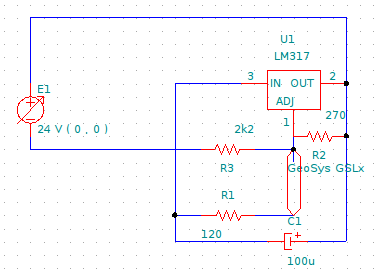
\includegraphics[width=0.5\hsize]{./images/schaltung-geosys-gslx.png}
\end{center}
\caption[Beschaltung des GeoSys GSLx, Quelle: Autoren]{\label{fig:schaltplangslx}Beschaltung des GeoSys GSLx, Quelle: Autoren}
\end{figure}

\subsection{Lichtmessung mittels Taos TSL2561}
\subsubsection{Initialisierung}
- set control reg: 03h --> power up, 7:2 ungenutzt
- set timing reg: 12h -- > gain 1 --> 16x, manual timing conroll 0, int time 10 --> 402 ms
\subsubsection{Beleuchtungsmessung}

\clearpage
\section{Versuchsanordnung}
Für die Durchführung der Messreihen wurde ein handelsübliches Papprohr mit
einer Länge von 120 cm und einem Durchmesser von 10 cm benutzt, wie es beispielsweise von der Post zum Versand genutzt wird. Dieses Rohr
kann auf beiden Seiten mit Kunststoffdeckeln verschlossen werden. Eine Seite
des Rohrs wurde so modifiziert, dass eine LED des LED-Moduls mit oder ohne
Optik eingesetzt werden kann. Der Deckel der gegenüberliegenden Seite wurde mit
3 Öffnungen versehen um die 3 Lichtsensoren einsetzen zu können.

\begin{figure}[h] 
  \subfigure[Deckel zur Aufnahme des LED-Moduls]{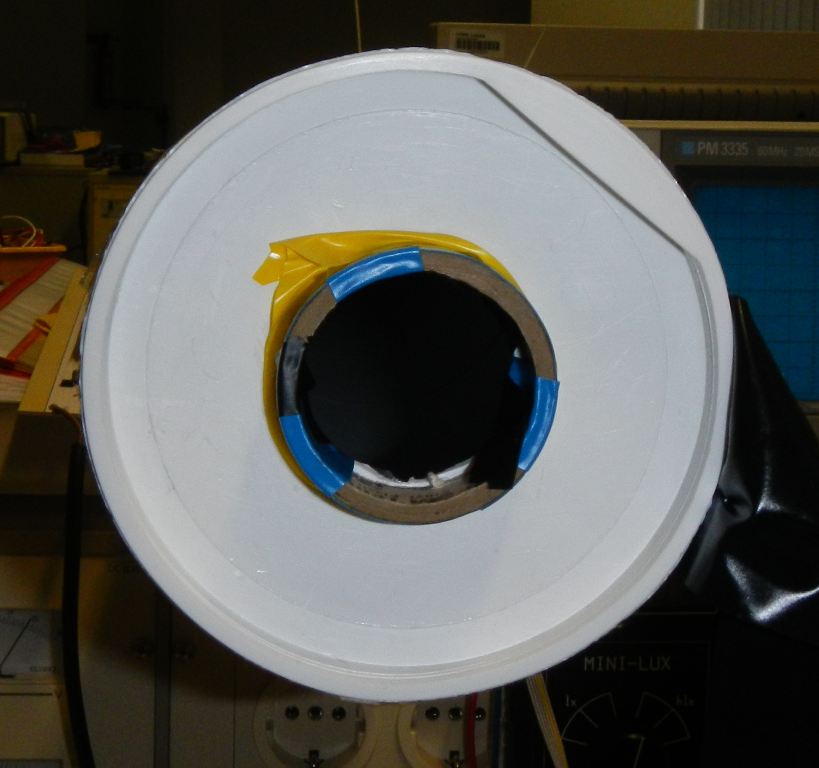
\includegraphics[width=0.495\textwidth]{./images/foto_hardware_beleuchtungsdeckel.png}} 
  \subfigure[Sensoren: MiniLux, GSLx,
TSL2561]{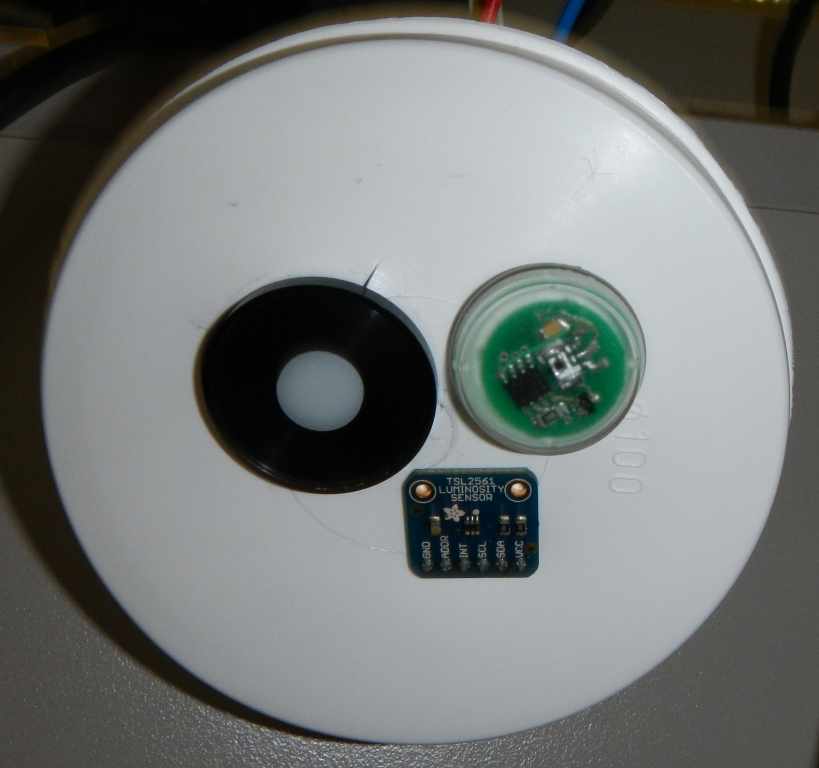
\includegraphics[width=0.495\textwidth]{./images/foto_hardware_sensordeckel.png}} 
  \subfigure[Messrohr]{\includegraphics[width=1\hsize]{./images/foto_hardware_messrohr.png}}
  \caption[Messaufbau]{\label{fotohwmessaufbau}Messaufbau, Quelle: Autoren}
\end{figure} 

Um bei der Bestimmung der Messreihen tragfähige Ergebnisse zu generieren, wurde jede einzelne Messung mit der Messgeräten parallel durchgeführt. Die beiden
Sensoren GeoSys GSLx und Taos TSL2561 wurden über einen Adapter mit dem Mikrocontroller LPC1768 verbunden und während der Messreihen von diesem ausgelesen.
Zusätzlich wurde noch ein kalibriertes Luxmeter MiniLux händisch ausgewertet um die Messwerte vergleichen und beurteilen zu können. 

Besonders hervorzuheben ist noch der Zusammenhang der Messergebnisse in Abhängigkeit der Geometrie sowie der Beschaffenheit der Innenseite des im Versuchsaufbau
verwendeten Papprohrs. Die Oberfläche dieser Innenseite ist weiß und reflektiert somit sehr viel auftreffendes Licht. Es ist davon auszugehen das bei der
Variation dieser Parameter andere Messergebnisse resultieren.

\clearpage
\section{Messergebnisse und Auswertung}
Die Messungen erfolgten in vier Messereihen, wobei die LED-Module mit 350mA und 500mA jeweils mit den Optiken Titanium-O-M und Titanium-O-SS kombiniert wurden.
Die Auflösung des PWM-Controllers beträgt 12 Bit, womit die PWM-Stufen 0 bis 4095 abgebildet werden können. Zusätzlich existiert noch eine Einstellung in
welcher der jeweilige PWM-Ausgang dauerhaft auf logisch 1 gesetzt wird. Für die Messreihen wurde im Bezug auf die PWM-Stufen eine Granularität von 100 gewählt.
Für jede Messreihe wurden Messwerte  des Sensors Taos TSL2561, des Luxmeters Mini-Lux sowie die Stromaufnahme des Messaufbaus aufgenommen.
Abschließend wurde noch eine Messreihe zur Stromaufnahme des komplett bestückten Straßenlampenprototypen aufgebnommen.

\subsection{LED-Modul 350mA mit Optik Titanium-O-M}

\begin{figure}[H]
  \begin{center}
    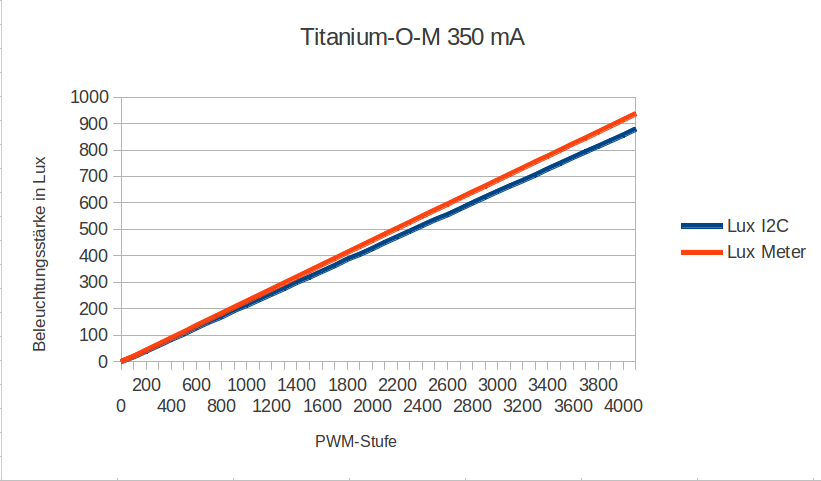
\includegraphics[width=1\hsize]{./images/350-m-print.png}
  \end{center}
\caption[Diagramm zur Messreihe LED-Modul 350mA mit Optik Titanium-O-M]{\label{diagram350matitm}Diagramm zur Messreihe LED-Modul 350mA mit Optik
Titanium-O-M.}
\end{figure}

\begin{longtable}[H]
{p{35mm}>{\columncolor[gray]{0.97}}p{35mm}p{35mm}}
  \rowcolor[gray]{.9}
    \textbf{PWM-Wert} & \textbf{TSL2561 [Lux]} & \textbf{Mini-Lux [Lux]} \\ 

    0 & 0 & 0 \\
\rowcolor[gray]{.95}
100	&	18	&	20	\\
200	&	39	&	43	\\
\rowcolor[gray]{.95}
300	&	61	&	66	\\
400	&	84	&	89	\\
\rowcolor[gray]{.95}
500	&	105	&	112	\\
600	&	128	&	136	\\
\rowcolor[gray]{.95}
700	&	149	&	159	\\
800	&	169	&	182	\\
\rowcolor[gray]{.95}
900	&	193	&	205	\\
1000	&	212	&	228	\\
\rowcolor[gray]{.95}
1100	&	234	&	251	\\
1200	&	255	&	274	\\
\rowcolor[gray]{.95}
1300	&	277	&	297	\\
1400	&	300	&	320	\\
\rowcolor[gray]{.95}
1500	&	319	&	343	\\
1600	&	341	&	366	\\
\rowcolor[gray]{.95}
1700	&	362	&	389	\\
1800	&	386	&	412	\\
\rowcolor[gray]{.95}
1900	&	405	&	435	\\
2000	&	427	&	458	\\
\rowcolor[gray]{.95}
2100	&	450	&	481	\\
2200	&	471	&	504	\\
\rowcolor[gray]{.95}
2300	&	493	&	527	\\
2400	&	515	&	550	\\
\rowcolor[gray]{.95}
2500	&	536	&	573	\\
2600	&	555	&	595	\\
\rowcolor[gray]{.95}
2700	&	577	&	618	\\
2800	&	600	&	641	\\
\rowcolor[gray]{.95}
2900	&	622	&	663	\\
3000	&	643	&	686	\\
\rowcolor[gray]{.95}
3100	&	665	&	709	\\
3200	&	685	&	732	\\
\rowcolor[gray]{.95}
3300	&	705	&	755	\\
3400	&	729	&	777	\\
\rowcolor[gray]{.95}
3500	&	750	&	800	\\
3600	&	771	&	823	\\
\rowcolor[gray]{.95}
3700	&	793	&	845	\\
3800	&	814	&	868	\\
\rowcolor[gray]{.95}
3900	&	835	&	891	\\
4000	&	856	&	914	\\
\rowcolor[gray]{.95}
4095	&	879	&	937	\\
4096\_voll	&	879	&	937	\\
\caption{Messreihe LED-Modul 350mA mit Optik Titanium-O-M}
\label{tab:350maTitM}
\end{longtable}

%%%%%%%%%%%%%%%%%%%%%%%%%%%%%%%%%%%%%%%%%%%%%%%%%%%%%%%%%%%%%%

\subsection{LED-Modul 350mA mit Optik Titanium-O-SS}

\begin{figure}[H]
  \begin{center}
    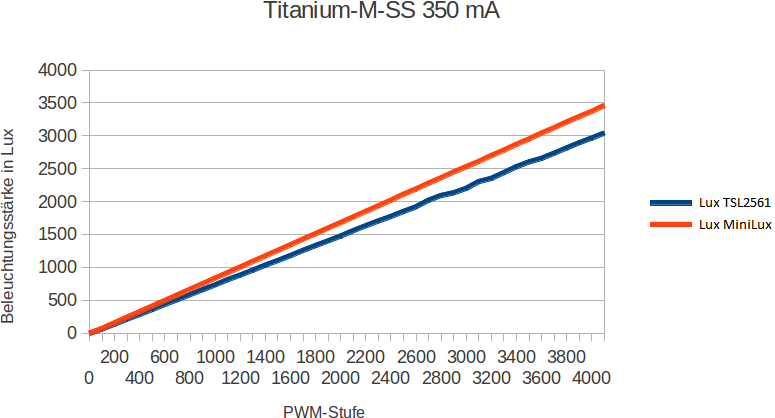
\includegraphics[width=1\hsize]{./images/350-ss-print.png}
  \end{center}
\caption[Diagramm zur Messreihe LED-Modul 350mA mit Optik Titanium-O-SS]{\label{diagram350matitss}Diagramm zur Messreihe LED-Modul 350mA mit Optik
Titanium-O-SS.}
\end{figure}

\begin{longtable}[H]{p{35mm}>{\columncolor[gray]{0.97}}p{35mm}p{35mm}}
  \rowcolor[gray]{.9}
    \textbf{PWM-Wert} & \textbf{TSL2561 [Lux]} & \textbf{Mini-Lux [Lux]} \\ 
0 & 0 & 0 \\
0	&	0	&	0	\\
100	&	63	&	73	\\
200	&	140	&	158	\\
300	&	213	&	243	\\
400	&	287	&	328	\\
500	&	361	&	413	\\
600	&	438	&	497	\\
700	&	510	&	582	\\
800	&	586	&	666	\\
900	&	661	&	751	\\
1000	&	733	&	836	\\
1100	&	813	&	920	\\
1200	&	882	&	1005	\\
1300	&	958	&	1090	\\
1400	&	1034	&	1174	\\
1500	&	1105	&	1259	\\
1600	&	1179	&	1343	\\
1700	&	1257	&	1428	\\
1800	&	1332	&	1512	\\
1900	&	1402	&	1597	\\
2000	&	1476	&	1681	\\
2100	&	1558	&	1766	\\
2200	&	1634	&	1850	\\
2300	&	1705	&	1935	\\
2400	&	1774	&	2020	\\
2500	&	1850	&	2110	\\
2600	&	1920	&	2190	\\
2700	&	2020	&	2280	\\
2800	&	2093	&	2360	\\
2900	&	2134	&	2450	\\
3000	&	2200	&	2530	\\
3100	&	2304	&	2610	\\
3200	&	2353	&	2700	\\
3300	&	2440	&	2780	\\
3400	&	2530	&	2870	\\
3500	&	2602	&	2950	\\
3600	&	2657	&	3040	\\
3700	&	2733	&	3120	\\
3800	&	2815	&	3210	\\
3900	&	2893	&	3290	\\
4000	&	2965	&	3370	\\
4095	&	3042	&	3460	\\
4096\_voll	&	3041	&	3460	\\
\caption{Messreihe LED-Modul 350mA mit Optik Titanium-O-SS}
\label{tab:350maTitSS}
\end{longtable}

%%%%%%%%%%%%%%%%%%%%%%%%%%%%%%%%%%%%%%%%%%%%%%%%%%%%%%%%%%%%%%%

\subsection{LED-Modul 500mA mit Optik Titanium-O-M}

\begin{figure}[H]
  \begin{center}
    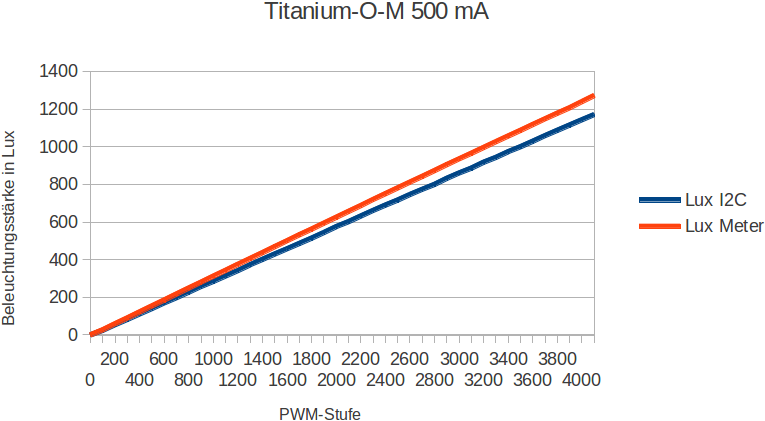
\includegraphics[width=1\hsize]{./images/500-m-print.png}
  \end{center}
\caption[Diagramm zur Messreihe LED-Modul 500mA mit Optik Titanium-O-M]{\label{diagram500matitm}Diagramm zur Messreihe LED-Modul 500mA mit Optik
Titanium-O-M.}
\end{figure}

\begin{longtable}[H]{p{35mm}>{\columncolor[gray]{0.97}}p{35mm}p{35mm}}
  \rowcolor[gray]{.9}
    \textbf{PWM-Wert} & \textbf{TSL2561 [Lux]} & \textbf{Mini-Lux [Lux]} \\ 
0 & 0 & 0 \\
\rowcolor[gray]{.95}
100 & 24 & 27 \\
200 & 53 & 59 \\
\rowcolor[gray]{.95}
300 & 82 & 90 \\
400 & 111 & 122 \\
\rowcolor[gray]{.95}
500 & 140 & 154 \\
600 & 169 & 185 \\
\rowcolor[gray]{.95}
700 & 198 & 217 \\
800 & 227 & 249 \\
\rowcolor[gray]{.95}
900 & 257 & 280 \\
1000 & 284 & 312 \\
\rowcolor[gray]{.95}
1100 & 313 & 343 \\
1200 & 342 & 375 \\
\rowcolor[gray]{.95}
1300 & 372 & 406 \\
1400 & 401 & 437 \\
\rowcolor[gray]{.95}
1500 & 430 & 469 \\
1600 & 457 & 500 \\
\rowcolor[gray]{.95}
1700 & 486 & 532 \\
1800 & 514 & 562 \\
\rowcolor[gray]{.95}
1900 & 544 & 594 \\
2000 & 575 & 625 \\
\rowcolor[gray]{.95}
2100 & 601 & 656 \\
2200 & 631 & 687 \\
\rowcolor[gray]{.95}
2300 & 661 & 719 \\
2400 & 690 & 750 \\
\rowcolor[gray]{.95}
2500 & 716 & 781 \\
2600 & 746 & 812 \\
\rowcolor[gray]{.95}
2700 & 773 & 842 \\
2800 & 800 & 873 \\
\rowcolor[gray]{.95}
2900 & 832 & 905 \\
3000 & 860 & 935 \\
\rowcolor[gray]{.95}
3100 & 886 & 965 \\
3200 & 917 & 996 \\
\rowcolor[gray]{.95}
3300 & 943 & 1027 \\
3400 & 974 & 1057 \\
\rowcolor[gray]{.95}
3500 & 1000 & 1087 \\
3600 & 1029 & 1118 \\
\rowcolor[gray]{.95}
3700 & 1059 & 1148 \\
3800 & 1087 & 1178 \\
\rowcolor[gray]{.95}
3900 & 1115 & 1207 \\
4000 & 1144 & 1240 \\
\rowcolor[gray]{.95}
4095 & 1173 & 1272 \\
4096\_voll & 1174 & 1274 \\
\caption{Messreihe LED-Modul 500mA mit Optik Titanium-O-M}
\label{tab:500maTitM}
\end{longtable}

%%%%%%%%%%%%%%%%%%%%%%%%%%%%%%%%%%%%%%%%%%%%%%%%%%%%%%%%%%%%%%%%%%%%%%%%%

\subsection{LED-Modul 500mA mit Optik Titanium-O-SS}

\begin{figure}[H]
  \begin{center}
    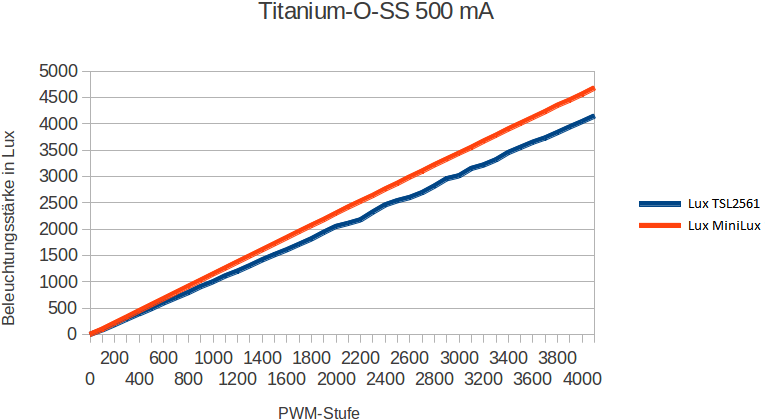
\includegraphics[width=1\hsize]{./images/500-ss-print.png}
  \end{center}
\caption[Diagramm zur Messreihe LED-Modul 500mA mit Optik Titanium-O-SS]{\label{diagram500matitss}Diagramm zur Messreihe LED-Modul 500mA mit Optik
Titanium-O-SS.}
\end{figure}

\begin{longtable}[H]{p{35mm}>{\columncolor[gray]{0.97}}p{35mm}p{35mm}}
  \rowcolor[gray]{.9}
    \textbf{PWM-Wert} & \textbf{TSL2561 [Lux]} & \textbf{Mini-Lux [Lux]} \\ 
0	&	0	&	0	\\
\rowcolor[gray]{.95}
100	&	85	&	99	\\
200	&	187	&	216	\\
\rowcolor[gray]{.95}
300	&	292	&	332	\\
400	&	390	&	449	\\
\rowcolor[gray]{.95}
500	&	491	&	565	\\
600	&	600	&	681	\\
\rowcolor[gray]{.95}
700	&	695	&	797	\\
800	&	796	&	913	\\
\rowcolor[gray]{.95}
900	&	908	&	1029	\\
1000	&	999	&	1145	\\
\rowcolor[gray]{.95}
1100	&	1111	&	1261	\\
1200	&	1202	&	1377	\\
\rowcolor[gray]{.95}
1300	&	1306	&	1493	\\
1400	&	1416	&	1608	\\
\rowcolor[gray]{.95}
1500	&	1514	&	1723	\\
1600	&	1608	&	1839	\\
\rowcolor[gray]{.95}
1700	&	1709	&	1955	\\
1800	&	1814	&	2070	\\
\rowcolor[gray]{.95}
1900	&	1938	&	2180	\\
2000	&	2050	&	2300	\\
\rowcolor[gray]{.95}
2100	&	2108	&	2420	\\
2200	&	2176	&	2530	\\
\rowcolor[gray]{.95}
2300	&	2323	&	2640	\\
2400	&	2459	&	2760	\\
\rowcolor[gray]{.95}
2500	&	2541	&	2870	\\
2600	&	2600	&	2990	\\
\rowcolor[gray]{.95}
2700	&	2691	&	3100	\\
2800	&	2817	&	3220	\\
\rowcolor[gray]{.95}
2900	&	2956	&	3330	\\
3000	&	3011	&	3440	\\
\rowcolor[gray]{.95}
3100	&	3150	&	3550	\\
3200	&	3218	&	3670	\\
\rowcolor[gray]{.95}
3300	&	3315	&	3780	\\
3400	&	3452	&	3900	\\
\rowcolor[gray]{.95}
3500	&	3551	&	4010	\\
3600	&	3650	&	4120	\\
\rowcolor[gray]{.95}
3700	&	3729	&	4230	\\
3800	&	3832	&	4350	\\
\rowcolor[gray]{.95}
3900	&	3940	&	4450	\\
4000	&	4039	&	4560	\\
\rowcolor[gray]{.95}
4095	&	4147	&	4680	\\
4096\_voll	&	4147	&	4680	\\
\caption{Messreihe LED-Modul 500mA mit Optik Titanium-O-SS}
\label{tab:500maTitSS}
\end{longtable}

%%%%%%%%%%%%%%%%%%%%%%%%%%%%%%%%%%%%%%%%%%%%%%%%%%%%%%%%%%%%%%%%%%%%

\subsection{Leistungsaufnahme der LED-Module während der Messreihen}

\begin{figure}[H]
  \begin{center}
    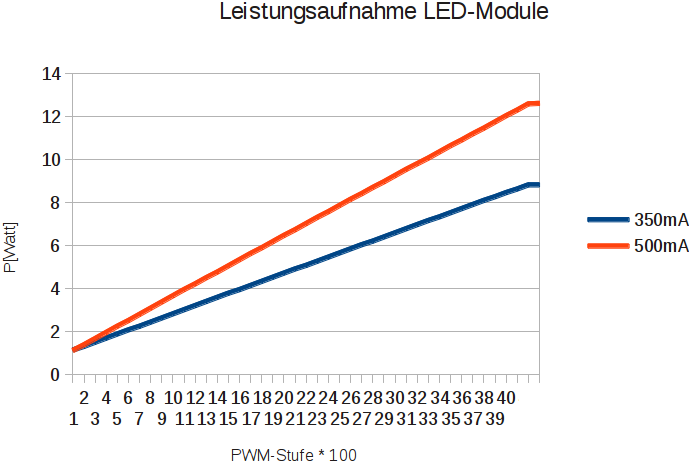
\includegraphics[width=1\hsize]{./images/350-500-leistungsaufnahme.png}
  \end{center}
\caption[Diagramm zur Leistungsaufnahme der LED-Module während der Messreihen]{\label{diagramPled}Diagramm zur Leistungsaufnahme der LED-Module während der
Messreihen.}
\end{figure}

\begin{longtable}[H]{p{35mm}>{\columncolor[gray]{0.97}}p{35mm}p{35mm}}
  \rowcolor[gray]{.9}
    \textbf{PWM-Wert} & \textbf{P LED-Modul 350mA [Watt]} & \textbf{P LED-Modul 500mA [Watt]} \\ 
0	&	0,0816	&	1,128	\\
\rowcolor[gray]{.95}
100	&	0,2136	&	1,392	\\
200	&	0,432	&	1,68	\\
\rowcolor[gray]{.95}
300	&	0,5256	&	1,968	\\
400	&	0,5328	&	2,256	\\
\rowcolor[gray]{.95}
500	&	0,5688	&	2,52	\\
600	&	0,7536	&	2,808	\\
\rowcolor[gray]{.95}
700	&	0,8568	&	3,096	\\
800	&	0,9624	&	3,384	\\
\rowcolor[gray]{.95}
900	&	1,0656	&	3,672	\\
1000	&	1,1664	&	3,96	\\
\rowcolor[gray]{.95}
1100	&	1,2744	&	4,224	\\
1200	&	1,3776	&	4,512	\\
\rowcolor[gray]{.95}
1300	&	1,4808	&	4,776	\\
1400	&	1,584	&	5,064	\\
\rowcolor[gray]{.95}
1500	&	1,6872	&	5,352	\\
1600	&	1,7928	&	5,64	\\
\rowcolor[gray]{.95}
1700	&	1,896	&	5,904	\\
1800	&	1,9992	&	6,192	\\
\rowcolor[gray]{.95}
1900	&	2,1024	&	6,48	\\
2000	&	2,208	&	6,744	\\
\rowcolor[gray]{.95}
2100	&	2,3136	&	7,032	\\
2200	&	2,388	&	7,32	\\
\rowcolor[gray]{.95}
2300	&	2,5224	&	7,584	\\
2400	&	2,628	&	7,872	\\
\rowcolor[gray]{.95}
2500	&	2,736	&	8,16	\\
2600	&	2,8392	&	8,424	\\
\rowcolor[gray]{.95}
2700	&	2,9448	&	8,712	\\
2800	&	3,0552	&	8,976	\\
\rowcolor[gray]{.95}
2900	&	3,1464	&	9,264	\\
3000	&	3,2664	&	9,552	\\
\rowcolor[gray]{.95}
3100	&	3,3696	&	9,816	\\
3200	&	3,4752	&	10,08	\\
\rowcolor[gray]{.95}
3300	&	3,5832	&	10,368	\\
3400	&	3,6888	&	10,656	\\
\rowcolor[gray]{.95}
3500	&	3,7992	&	10,92	\\
3600	&	3,9048	&	11,208	\\
\rowcolor[gray]{.95}
3700	&	4,0104	&	11,472	\\
3800	&	4,1184	&	11,76	\\
\rowcolor[gray]{.95}
3900	&	4,2264	&	12,048	\\
4000	&	4,332	&	12,312	\\
\rowcolor[gray]{.95}
4095	&	4,4544	&	12,6	\\
4096\_voll	&	4,4544	&	12,624	\\
\caption{Leistungsaufnahme der LED-Module während der Messreihen}
\label{tab:pledmodule}
\end{longtable}
%%%%%%%%%%%%%%%%%%%%%%%%%%%%%%%%%%%%%%%%%%%%%%%%%%%%%%%%%%%%%%%%%%%%

\subsection{Leistungsaufnahme des Straßenlampen-Prototypen}

\begin{figure}[H]
  \begin{center}
    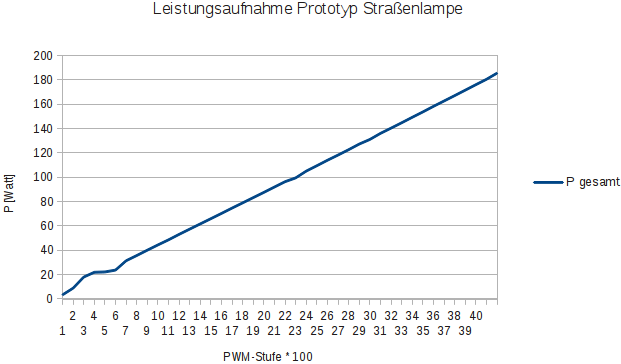
\includegraphics[width=1\hsize]{./images/prototyp-leistungsaufnahme.png}
  \end{center}
\caption[Diagramm zur Leistungsaufnahme des Straßenlampen-Prototyps.]{\label{diagramPprototyp}Diagramm zur Leistungsaufnahme des Straßenlampen-Prototyps.}
\end{figure}

\begin{longtable}[H]{p{35mm}>{\columncolor[gray]{0.97}}p{35mm}}
  \rowcolor[gray]{.9}
    \textbf{PWM-Wert} & \textbf{P Prototyp [Watt]}\\ 
0	&	3,4	\\
\rowcolor[gray]{.95}
100	&	8,9	\\
200	&	18	\\
\rowcolor[gray]{.95}
300	&	21,9	\\
400	&	22,2	\\
\rowcolor[gray]{.95}
500	&	23,7	\\
600	&	31,4	\\
\rowcolor[gray]{.95}
700	&	35,7	\\
800	&	40,1	\\
\rowcolor[gray]{.95}
900	&	44,4	\\
1000	&	48,6	\\
\rowcolor[gray]{.95}
1100	&	53,1	\\
1200	&	57,4	\\
\rowcolor[gray]{.95}
1300	&	61,7	\\
1400	&	66	\\
\rowcolor[gray]{.95}
1500	&	70,3	\\
1600	&	74,7	\\
\rowcolor[gray]{.95}
1700	&	79	\\
1800	&	83,3	\\
\rowcolor[gray]{.95}
1900	&	87,6	\\
2000	&	92	\\
\rowcolor[gray]{.95}
2100	&	96,4	\\
2200	&	99,5	\\
\rowcolor[gray]{.95}
2300	&	105,1	\\
2400	&	109,5	\\
\rowcolor[gray]{.95}
2500	&	114	\\
2600	&	118,3	\\
\rowcolor[gray]{.95}
2700	&	122,7	\\
2800	&	127,3	\\
\rowcolor[gray]{.95}
2900	&	131,1	\\
3000	&	136,1	\\
\rowcolor[gray]{.95}
3100	&	140,4	\\
3200	&	144,8	\\
\rowcolor[gray]{.95}
3300	&	149,3	\\
3400	&	153,7	\\
\rowcolor[gray]{.95}
3500	&	158,3	\\
3600	&	162,7	\\
\rowcolor[gray]{.95}
3700	&	167,1	\\
3800	&	171,6	\\
\rowcolor[gray]{.95}
3900	&	176,1	\\
4000	&	180,5	\\
\rowcolor[gray]{.95}
4095	&	185,6	\\
4096\_voll	&	185,6	\\
\caption{Leistungsaufnahme des Straßenlampen-Prototyps.}
\label{tab:pprototyp}
\end{longtable}

    
    
\clearpage
\section{Schlussbetrachtung}
Anhand der Messreihen in der Messkonstruktion wird ein linearer Zusammenhang zwischen den PWM-Stufen und den zugehörigen gemessenen Beleuchtungsstärken
ersichtlich. Es soll jedoch nochmals darauf hingewiesen werden, dass alle oben genannten Messwerte nur für den in diesem Dokument beschriebenen Messaufbau
Gültigkeit besitzen.

%% Tabelle
%\vspace*{1cm}
%\begin{longtable}{p{34mm}>{\columncolor[gray]{0.97}}p{33mm}p{33mm}>{\columncolor[gray]{0.97}}p{33mm}}
%\rowcolor[gray]{.9}Funktion & \textbf{IPCop} & \textbf{IPFire} & \textbf{pfSense}\\
%Lizenz & GPL\cite{GPLLicense} & GPL\cite{GPLLicense} & BSD\cite{FreeBSDLicense}\\
%\rowcolor[gray]{.95}Betriebssystem & Linux & Linux & FreeBSD   \\
%Hardware"-architektur & i386, Cobald, Sparc, PowerPC & i386, AMD64 & i386, AMD64\\
%\caption{Merkmale ausgew\"ahlter Routerdistributionen im Vergleich}
%\label{Merkmale der Routerdistributionen im Vergleich}
%\end{longtable}

\clearpage
\section{Schluss}
Dies ist der Schlussteil. Abschlie\ss{}ende Empfehlung

\section{Anhang}
\subsection{Quellcodelisting}
\definecolor{listinggray}{gray}{0.9}
\definecolor{lbcolor}{rgb}{0.9,0.9,0.9}
\lstset{
	language=C,
	keywordstyle=\bfseries\ttfamily\color[rgb]{0,0,1},
	identifierstyle=\ttfamily,
	commentstyle=\color[rgb]{0.133,0.545,0.133},
	stringstyle=\ttfamily\color[rgb]{0.627,0.126,0.941},
	showstringspaces=false,
	basicstyle=\scriptsize,
	numbers=left,
	stepnumber=1,
	numbersep=6pt,
	numberstyle=\tiny,
	tabsize=2,
	breaklines=true,	%automatischer Zeilenumbruch
	prebreak = \raisebox{0ex}[0ex][0ex]{\ensuremath{\hookleftarrow}},
	breakatwhitespace=false,
	aboveskip={1.5\baselineskip},
  	columns=fixed,
  	upquote=true,
  	extendedchars=true,
  	backgroundcolor=\color[rgb]{0.95,0.95,0.95},
}
\begin{lstlisting}[captionpos=b, caption=MBED-Programmcode für den Messaufbau, label=messprogkomplett]
#include "mbed.h"
#include "string"

AnalogIn ain(p15);              //Lichtsensor GeoSys
Serial serterm(USBTX, USBRX);   //serielles Terminal zum PC

DigitalOut led1(LED1);
DigitalOut led2(LED2);
DigitalOut led3(LED3);
DigitalOut led4(LED4);

DigitalOut oe(p18);

I2C i2c(p9, p10);        // sda, scl

LocalFileSystem local("local");

Timer t;

const int buffersize = 100;
const int tslWriteAddr = 0x52;
const int tslReadAddr  = 0x53;
const int pwmWriteAddr = 0x80;
const int pwmReadAddr  = 0x81;

int pwmVal[16];

int ledStart(int times, double delay)
{
    int i;

    led1 = 0;
    led2 = 0;
    led3 = 0;
    led4 = 0;

    for(i = 0; i < times; i++) {
        led1 = 1;
        wait(delay);
        led1 = 0;
        led2 = 1;
        wait(delay);
        led2 = 0;
        led3 = 1;
        wait(delay);
        led3 = 0;
        led4 = 1;
        wait(delay);
        led4 = 0;
    }
    wait(delay);
    return 0;
}

int setLed(int led)
{
    led1 = led & 1;
    led2 = led >> 1 & 1;
    led3 = led >> 2 & 1;
    led4 = led >> 3 & 1;

    return 0;
}

void readText(int size, char *buf)
{
    char temp;
    int i = 0;

    buf = (char *)malloc(100*sizeof(char));

    while(i < size && ((temp = serterm.getc()) != '\r')) {
        buf[i++] = temp;
        serterm.putc(temp);
    }
    buf[i] = '\0';
}

int swReset()
{
    char cmd[1];
    cmd[0] = 0x06;
    i2c.write(0x00,cmd,1);
    return 0;
}

int setPwm12(int n, int ontime)
{
    char baseAddr;
    char cmd[5];
    int start, stop;

    // calulate delay time
    if(n == 0)
        start = 0;
    else
        start = n * 256;

    // calulate stop time
    stop = start + ontime;

    // address calculation for channel n
    if(n == 16) {               // all call address
        baseAddr = 0xfa;
    } else if(n >= 0 && n <= 15) {
        baseAddr = n  * 4 + 0x06;
    } else {
        return 1;
    }

    if(ontime < 0 && ontime > 4096) {
        return 2;
    }

    if(ontime == 4096) {        // LED Full ON
        cmd[0] = baseAddr;
        cmd[1] = 0x00;
        cmd[2] = 0x10;          // full on bit 4 set
        cmd[3] = 0x00;
        cmd[4] = 0x00;
    } else {                    // variable brightness
        if(stop > 4095) {
            stop = stop - 4096;
        }
        cmd[0] = baseAddr;          // start address for channel
        cmd[1] = start & 0xff;      // LED_ON_LOW
        cmd[2] = start >> 8 & 0x0f; // LED_ON_HIGH
        cmd[3] = stop & 0xff;       // LED_OFF_LOW
        cmd[4] = stop >> 8 & 0x0f;  // LED_OFF_HIGH
    }

    i2c.write(pwmWriteAddr, cmd, 5);

    if(n!=16)
        pwmVal[n] = ontime;

    return 0;
}

int readPwm12(int n)
{
    char baseAddr;
    char cmd[5];
    char read[16];
    int start, stop, val;

    // address calculation for channel n
if(n == 16) {               // all call address
        baseAddr = 0xfa;
    } else if(n >= 0 && n <= 15) {
        baseAddr = n  * 4 + 0x06;
    } else {
        return 1;
    }

    cmd[0] = baseAddr;
    i2c.write(pwmWriteAddr, cmd, 1);
    i2c.read(pwmReadAddr, read, 4);
    start = read[0] + (read[1] << 8);
    stop = read[2] + (read[3] << 8);
    if(stop < start)
        stop += 4096;
    val = stop - start;
    return val;
}

int initPwm(int mode)
{
    int i;
    char cmd[2];

    for(i = 0; i <= 15; i++) {
        pwmVal[i] = 0;
    }

    // set i2c clock to fast mode
    i2c.frequency(400000);

    // set MODE1 register
    cmd[0] = 0x00;
    cmd[1] = 0x00;

    i2c.write(pwmWriteAddr, cmd, 2);

    // set MODE2 register
    cmd[0] = 0x01;
    cmd[1] = 0x04;

    i2c.write(pwmWriteAddr, cmd, 2);

    // set MODE1 register
    // set AI flag
    cmd[0] = 0x00;
    cmd[1] = 0x20;

    i2c.write(pwmWriteAddr, cmd, 2);

    // set all pwm channels to 0
    setPwm12(16, 0);

    //output enable of pwm controller
    oe = 0;



    return 0;
}

int initTsl()
{
    char cmd[5];

    // set control register - powering up
    cmd[0] = 0x80;
    cmd[1] = 0x03;
    i2c.write(tslWriteAddr, cmd, 2);

    // set timing register - high gain and 402 ms integration time
    cmd[0] = 0x81;
    cmd[1] = 0x12;
    i2c.write(tslWriteAddr, cmd, 2);

    return 0;
}

int initDS18S20()
{

    return 0;
}

double readLux()
{
    double lux, dif;
    // full range
    int ch0;
    // ir only
    int ch1;
    char cmd[5];

    //channel 0 - full range
    cmd[0] = 0x8C;
    i2c.write(tslWriteAddr, cmd, 1);
    i2c.read(tslReadAddr, cmd, 2);

    ch0 = cmd[1] << 8;
    ch0 = ch0 + cmd[0];

    // channel 1 - ir only
    cmd[0] = 0x8e;
    i2c.write(tslWriteAddr, cmd, 1);
    i2c.read(tslReadAddr, cmd, 2);

    ch1 = cmd[1] << 8;
    ch1 = ch1 + cmd[0];

    dif = ch1/ch0;

    if(dif <= 0.50) {
        lux = 0.0304 * ch0 - 0.062 * ch0 * pow(ch1/ch0, 1.4);
    } else if (dif <= 0.61) {
        lux = 0.0224 * ch0 - 0.031 * ch1;
    } else if (dif <= 0.80) {
        lux = 0.0128 * ch0 - 0.0153 * ch1;
    } else if (dif <= 1.3) {
        lux = 0.00146 * ch0 - 0.00112 * ch1;
    } else if (dif > 0) {
        lux = 0;
    } else {
        return -1.0;
    }

    return lux;
}

double readLuxScale()
{
    char cmd[5];
    double lux;
    lux = readLux();
    if (lux > 1900.0) {
        //reduce integration time to 101 ms
        cmd[0] = 0x81;
        cmd[1] = 0x11;
        i2c.write(tslWriteAddr, cmd, 2);
        wait(1);

        //meassure
        lux = readLux();

        //reset integration time
        cmd[0] = 0x81;
        cmd[1] = 0x12;
        i2c.write(tslWriteAddr, cmd, 2);
        wait(1);

        //scale value
        lux = lux / 0.252 * 1.0;
    }
    return lux;
}

double readLuxCalib()
{
    double baseVal = readLuxScale();
    return baseVal + baseVal * 0.1095;
}

void printHomeScreen()
{
    int i, j, bar;

    serterm.printf("\x1B[2J");    //VT100 erase screen
    serterm.printf("\x1B[H");     //VT100 home
    serterm.printf("AllInOne 0.2\n\rHomeScreen\n\r");
    serterm.printf("\n\rPWM Values:\n\r");
    for(i = 0; i <=15; i++) {
        pwmVal[i] = readPwm12(i);
        serterm.printf("channel %d: %d\r\x1B[46C[",i, pwmVal[i]);
        bar = pwmVal[i]/128+1;
        for(j = 0; j < 32; j++) {
            if(bar > 1 && j < bar)
                serterm.printf("=");
            else
                serterm.printf(" ");
        }
        serterm.printf("]\n\r");
    }
    serterm.printf("\n\rb - set brightness; o - options; m - measuring lux; s - measured series\n\r>");
}

int pwmDemo()
{
    int i, j;
//    for(j=0; j<=16; j++) {
    for(j=0; j<=1; j++) {
        setLed(j);
        for(i=0; i < 4096; i++) {
            setPwm12(j, i);
            wait(0.0005);
        }
        for(i=4096; i >= 0; i--) {
            setPwm12(j, i);
            wait(0.0005);
        }
    }
    setPwm12(0, 4096);
    wait(0.2);
    setPwm12(0,0);
    wait(0.2);
    setPwm12(0, 4096);
    wait(0.2);
    setPwm12(0,0);
    return 0;
}


int main()
{
    char charbuf[buffersize];
    char cmd[5];
    char temp;
    char filename[13];
    char path[50];
    int cap;
    double value;
    char charbuf2;

    wait(1);
    serterm.printf("\x1B[2J");    //VT100 erase screen
    serterm.printf("\x1B[H");     //VT100 home
    serterm.printf("Starting mbed...\n\r");

    // indicate controler strat
    ledStart(1, 0.1);

    setLed(15);

    wait(1);
    setLed(0);

    //i2c fast mode 400 kHz
    i2c.frequency(400000);
    setLed(1);

    // initialize pwm module
    initPwm(0);
    setLed(2);

    // initialize i2c TAOS Sensor
    initTsl();
    setLed(3);

    //pwmDemo();


    while(1) {
        printHomeScreen();
        temp = serterm.getc();
        switch(temp) {
            case 'b':
                int i = 0;
                int channel, brightness;
                serterm.printf("\x1B[2J");    //VT100 erase screen
                serterm.printf("\x1B[H");     //VT100 home

                for(i = 0; i<buffersize; i++)
                    charbuf[i] = '\0';
                i = 0;
                serterm.printf("\n\rSelect channel (0 - 15; 16 - all channels): ");
                while(i < 99 && ((temp = serterm.getc()) != '\r')) {
                    if((int)temp == 127) {
                        if(i > 0)
                            i--;
                    } else {
                        charbuf[i++] = temp;
                        serterm.putc(temp);
                    }
                }
                charbuf[i] = '\0';
                channel = atoi(charbuf);

                if(channel < 0 || channel > 16) {
                    serterm.printf("\n\rValue invalid\n\rHit any key to continue...\n\r");
                    serterm.getc();
                    break;
                }

                for(i = 0; i<buffersize; i++)
                    charbuf[i] = '\0';
                i = 0;
                serterm.printf("\n\rSet brightness (PWM: 0 - 4095; Full ON: 4096): ");
                while(i < 99 && ((temp = serterm.getc()) != '\r')) {
                    if((int)temp == 127) {
                        if(i > 0)
                            i--;
                    } else {
                        charbuf[i++] = temp;
                        serterm.putc(temp);
                    }
                }
                charbuf[i] = '\0';
                brightness = atoi(charbuf);

                if(brightness < 0 || brightness > 4096) {
                    serterm.printf("\n\rValue invalid\n\rHit any key to continue...\n\r");
                    serterm.getc();
                    break;
                }

                if(channel == 16) {
                    for(i = 0; i < 16; i++) {
                        setPwm12(i,brightness);
                    }
                } else {
                    setPwm12(channel,brightness);
                }
                break;

            case 'o':
                while(temp != 'q') {
                    serterm.printf("\x1B[2J");    //VT100 erase screen
                    serterm.printf("\x1B[H");     //VT100 home
                    serterm.printf("Options\n\r\n\r");
                    serterm.printf("TSL:\r\n");
                    serterm.printf("i - Integration time\r\n");
                    serterm.printf("\r\n");
                    serterm.printf("\r\n");
                    serterm.printf("\r\n");

                    serterm.printf("\r\n>");

                    temp = serterm.getc();

                    switch(temp) {
                        case 'i':
                            serterm.printf("\x1B[2J");    //VT100 erase screen
                            serterm.printf("\x1B[H");     //VT100 home
                            serterm.printf("Integration time\n\r\n\r");
                            break;
                        default:
                            break;
                    }
                }
                break;
            case 'm':
                while(temp != 'q') {
                    //int val;
                    double voltage, lux;
                    serterm.printf("\x1B[2J");    //VT100 erase screen
                    serterm.printf("\x1B[H");     //VT100 home
                    serterm.printf("Meassurement - hit 'q' for home screen - any key for refresh\n\n\r");

                    serterm.printf("TSL2561: %f Lux            \n\r",readLuxScale());
                    serterm.printf("TSL2561 (cal): %f Lux            \n\r",readLuxCalib());

                    //val = (int) ain.read_u16();
                    voltage = ain.read();
                    lux = 100/(0.8037-0.0806)*(voltage-0.1953);
                    serterm.printf("Geosys: %.10f V --> %f Lux             \n\r", voltage, lux);
                    temp = serterm.getc();
                }
                break;
            case 's':
                int stepSize, pause;
                serterm.printf("\x1B[2J");    //VT100 erase screen
                serterm.printf("\x1B[H");     //VT100 home

                // read filename
                serterm.printf("Enter filename: ");

                i = 0;
                while(i < 8 && ((temp = serterm.getc()) != '\r')) {
                    if((int)temp == 127) {
                        if(i > 0)
                            i--;
                    } else {
                        charbuf[i++] = temp;
                        serterm.putc(temp);
                    }
                }
                charbuf[i] = '\0';
                strcpy(filename, charbuf);
                strcat(filename, ".csv");
                strcpy(path, "/local/");
                strcat(path, filename);

                //read step size
                serterm.printf("\n\rEnter step size 0 - 500: ");
                i = 0;
                while(i < 8 && ((temp = serterm.getc()) != '\r')) {
                    if((int)temp == 127) {
                        if(i > 0)
                            i--;
                    } else {
                        charbuf[i++] = temp;
                        serterm.putc(temp);
                    }
                }
                charbuf[i] = '\0';
                stepSize = atoi(charbuf);
                if(stepSize < 0 || stepSize > 500) {
                    serterm.printf("\n\rInvalid value\n\r");
                    serterm.getc();
                    break;
                }

                //read step size
                serterm.printf("\n\rEnter pause time 0 - 10 (in full seconds): ");
                i = 0;
                while(i < 8 && ((temp = serterm.getc()) != '\r')) {
                    if((int)temp == 127) {
                        if(i > 0)
                            i--;
                    } else {
                        charbuf[i++] = temp;
                        serterm.putc(temp);
                    }
                }
                charbuf[i] = '\0';
                pause = atoi(charbuf);
                if(pause < 0 || pause > 10) {
                    serterm.printf("\n\rInvalid value\n\r");
                    serterm.getc();
                    break;
                }

                FILE *fp = fopen(path, "w");
                fprintf(fp, "pwmval;lux\n");
                serterm.printf("\n\rpwm --> lux\n\r");
                wait(1);
                for(i = 0; i < 4095; i+=stepSize) {
                    setPwm12(0, i);
                    wait(1);
                    value = readLuxScale();
                    fprintf(fp, "%d;%f\n",i ,value);
                    serterm.printf("%d --> %f\n\r",i ,value);
                    //serterm.getc();
                    setPwm12(0, 0);
                    wait(pause);
                    //serterm.getc();
                }
                if(stepSize >= 10) {
                    setPwm12(0, 4095);
                    wait(1);
                    value = readLuxScale();
                    fprintf(fp, "%d;%f\n",4095 ,value);
                    serterm.printf("%d --> %f\n\r",4095 ,value);
                    //serterm.getc();
                    setPwm12(0, 0);
                    wait(pause);
                    //serterm.getc();

                    setPwm12(0, 4095);
                    wait(1);
                    value = readLuxScale();
                    fprintf(fp, "%d;%f\n",4096 ,value);
                    serterm.printf("%d --> %f\n\r",4096 ,value);
                    //serterm.getc();
                    setPwm12(0, 0);
                    wait(pause);
                    //serterm.getc();
                }
                fclose(fp);
                serterm.printf("done...\n\r");
                setPwm12(0, 0);
                serterm.getc();
                break;
            case 't':
                while(((temp = serterm.getc()) != 'q')) {
                    for(i=0; i<=16; i++) {
                        serterm.printf("\n\rread %d: %d", i, readPwm12(i));
                    }
                }
                break;
            default:
                break;
        }
    }
}
\end{lstlisting}


\clearpage
\section{Glossar}
\begin{description}
 \item[I2C] Prtokoll zur Kommunikation in Ger\"aten
\end{description}

\clearpage
\section{Literatur- und Quellenverzeichnis}

\renewcommand\refname{Literaturverzeichnis}
\begin{thebibliography}{999}

\bibitem{buch_foobar}Michael W. Lucas:  {\sl Absolute BSD (2nd Edition). The Ultimate Guide to FreeBSD.} No Starch Press, 2008,
\\ISBN: 978-1-59327-151-0

\end{thebibliography}

\renewcommand\refname{Quellenverzeichnis}
\begin{thebibliography}{999}

%%\cite{citeverweis}
\bibitem{speci2c}
\url{http://www.nxp.com/documents/user_manual/UM10204.pdf}
\\Abrufbar am 10.03.2013

\bibitem{spec1wire}
\url{http://www.1wire.org}
\\Abrufbar am 10.03.2013

\bibitem{specled}
\url{http://www.osram-os.net/osram_os/CN/Downloads/Solid_State_Lighting/documents/LUW_W5AM_Pb-free_C_final.pdf}
\\Abrufbar am 10.03.2013

\bibitem{specpwm}
\url{http://www.nxp.com/documents/data_sheet/PCA9685.pdf}
\\Abrufbar am 11.03.2013

\bibitem{speclpc1768}
\url{http://www.nxp.com/documents/data_sheet/LPC1769_68_67_66_65_64_63.pdf}
\\Abrufbar am 11.03.2013

\bibitem{specminilux}
\url{http://www.mx-electronic.com/pdf/Bedienungsanleitungdeu.PDF}
\\Abrufbar am 11.03.2013

\bibitem{specds1820}
\url{http://www.systronix.com/Resource/ds1820.pdf}
\\Abrufbar am 11.03.2013

\end{thebibliography}

\clearpage
\section{Verzichtserkl\"arung}
\thispagestyle{plain}

Hiermit erkläre ich, dass ich die vorliegende Arbeit selbstständig und nur unter Verwendung der angegebenen Literatur und Hilfsmittel angefertigt habe.
Stellen, die wörtlich oder sinngemäß aus Quellen entnommen wurden, sind als solche
kenntlich gemacht.\\

Diese Arbeit wurde in gleicher oder ähnlicher Form noch keiner anderen Prüfungsbehörde vorgelegt.\\\\

Leipzig, \today
\end{document}
%% EOF